\documentclass{article}
\usepackage[spanish]{babel}
\usepackage{graphicx}

\title{Tratamiento} % Sets article title
\author{Noelia Barranco Godoy
\and Erik Zubimendi Solaguren\and
Elena Novillo Luceño}
\date{\today} % Sets date for date compiled


\begin{document} % All begin commands must be paired with an end command somewhere
    \begin{titlepage}
        \maketitle
        \thispagestyle{empty}
        \begin{center}
            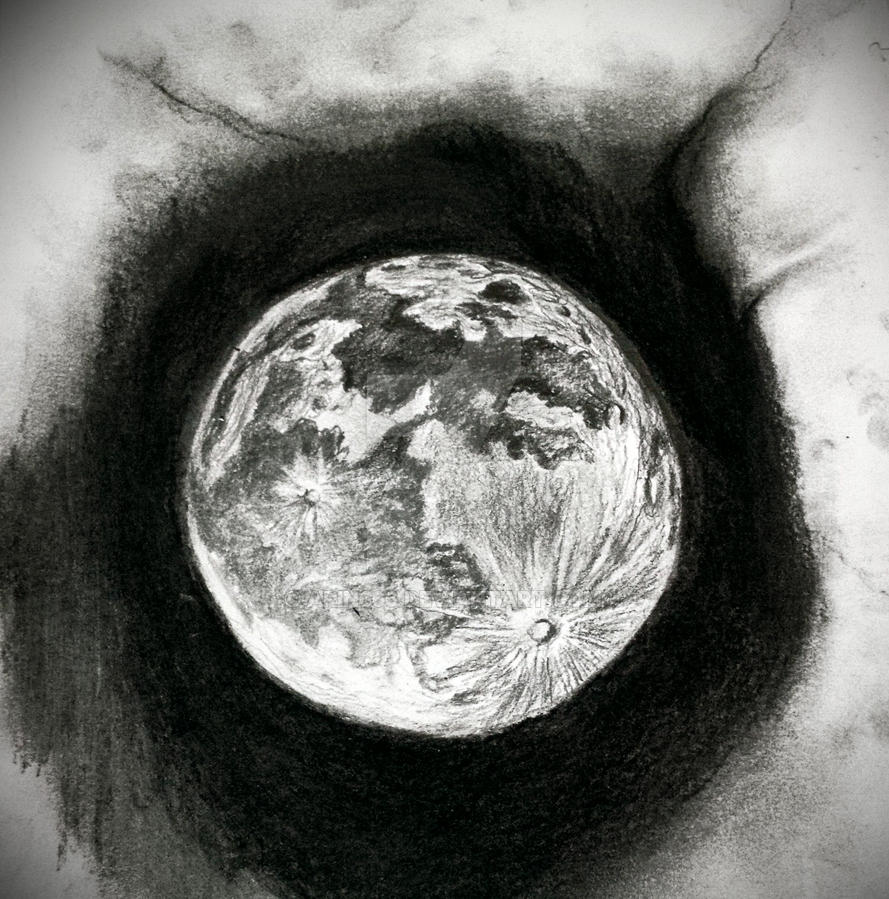
\includegraphics[scale=0.125]{moon.jpg}
        \end{center} 
    \end{titlepage}
        
    \tableofcontents
    \newpage
    
    \section{INTRODUCCIÓN}
    This section is just the game concept, updated with stakeholders’ feedback. Narrative and aesthetics have their own sub-section. Three pages long at most for the whole section.

    \subsection{CONCEPTO}
    \subsubsection{INFORMACIÓN BÁSICA}
    \begin{tabular}{||c|c||}
        \hline
        \textbf{Título} & Moonheir \\
        \textbf{Género} & RPG\\
        \textbf{Plataforma} & Navegador web\\
        \textbf{Público objetivo} & Jugadores casuales\\
        \hline
    \end{tabular}
    \subsubsection{DESCRIPCIÓN}
    This is the most important part. Most readers won’t really read past this point. You have at most two paragraphs to sell the idea. Maybe even three. Focus on:
    1. What is the game about?
    2. Why make this game instead of playing something else / something better?
    \subsubsection{CARACTERÍSTICAS PRINCIPALES}
    A list of the most important game features. We are going to expand on the mechanics later on, so be brief and don’t try to explain them in here.
    \subsubsection{RIESGOS}
    What are the main technical, artistic and market risks? How are they being addressed?


    \subsection{AMBIENTACIÓN}
    Tone and themes of the game.
    \subsubsection{ARTE}
    This is NOT a set of instructions for the art team. What are the GOALS of the art design? What are the constraints? What’s the game trying to convey? Remember to always use visual references.
    \subsubsection{MÚSICA Y SONIDOS}
    The same as above but for sound design. As there is no audio team, don’t sweat it. But remember to include audible references.  

    \newpage
    \section{MECÁNICAS}
    This section is a brief description of the game’s main mechanics. Which mechanics are appropriate heavily depends on the game concept. The following mechanics are a few candidates that usually will apply to most (single-player) games.

    Each mechanic should be about half-page long, and the whole section should be at most 5 pages long.
    \subsubsection{FLUJO DE JUEGO???} %TODO: Revisar traducción
    This one is easy: how do games start, how do they end, and what happens in between?

    \subsubsection{MUNDO DEL JUEGO}
    What are the main entities in the game world? How is the world constructed? What’s the camera doing and why? Usually will be heavily referenced in later descriptions.

    \subsubsection{JUGADOR}
    Who or what is the player? How does the player interact with the game world? If the player is customizable, how and why? Is there an inventory?

    \subsubsection{ENEMIGOS (Y NPC'S??)}
    Most games have enemies and/or NPCs. This section should give and idea about:
    a) Life Cycle: where do the come from and when do they dissapear?
    b) Behaviors: what are the general behaviors employed by them?

    \subsubsection{COMBATE}
    In some games, combat (which is just a specific interaction of the player with the enemies and environment) is the primary mechanic. If this is the case, then it deserves its own sub-section.

    \subsubsection{ITEMS/EQUIPO/CONSUMIBLES}
    There’s no point in listing all this stuff, unless the list is short. However, is important to give an idea of the variety (and how is it to be accomplished), placement and use.

    \subsubsection{ECONOMÍA}
    If the economy is an important part of the game, it must be described. Just an overview.

    \subsubsection{NARRATIVA}
    If the game has a significant narrative component, which mechanics are there to support the narrative intent? Things like dialogue trees, cutscenes and so on. Remember that voice overs are horrendously expensive.

    \subsubsection{OTROS}
    There is almost always some stuff that, while not  being important enough to deserve a proper explanation, is better being at least mentioned.


    \newpage
    \section{CONTENIDO DE MUESTRA}

    This section is the most important part from the point of view of the development team: how does all the previous stuff fit together? How does the game ACTUALLY play?

For most games, the ideal way of doing this is to design and describe a level, or at least a big enough chunk of one. It MUST include:
    a) Visual aids: almost always a map of some sort and...
    b) Entities and flow: ...an annotation of how the level is supposed to play out.

This section should be around 3 pages long.

\newpage
\section{INTERFAZ}
The point of this section is NOT to fully describe the game interfaces. It’s just an overview of the main problems and proposed solutions related to both the output and input interfaces. If the game’s interface is completely standard, this section should not exist or be very, very brief.

\subsection{GUI}

\subsection{CONTROLES}

\newpage
\section{REFERENCIAS} %Hay libreríasa de latex que ayudan con las citas

\end{document}
